\section{Thực nghiệm số}

\subsection{Mô hình và tham số}

Thực nghiệm được cài đặt bằng Python trên không gian $\mathcal{H}=\R$ với hàm mục tiêu
\[
F(x)=\frac{x^4}{4}.
\]
Nghiệm tối ưu là $x_{\star}=0$ và $F_{\star}=0$. Các tham số được chọn như sau:
\begin{equation}
x_0=4,
\qquad
A_0=1,
\qquad
\lambda_k=1,
\qquad
\varepsilon_k=\frac{0.2}{(k+1)^{7/4}},
\qquad
N=2000.
\label{eq:experiment-params}
\end{equation}
Cả ba phương pháp dùng cùng quy tắc
\begin{equation}
\alpha_k^2=(1-\alpha_k)A_k\lambda_k.
\label{eq:experiment-alpha}
\end{equation}
Đối với IAPPA2, \eqref{eq:experiment-alpha} tương ứng với việc chọn tỉ số trong điều kiện tham số bằng $1$, hợp lệ với $a=1$. Nhờ đó, khác biệt quan sát được không đến từ cách chọn $\alpha_k$.

Điểm cận kề là nghiệm duy nhất của phương trình
\[
z^3+z-y=0.
\]
Nghiệm này được tính bằng phương pháp Newton, dừng khi bước hiệu chỉnh nhỏ hơn $10^{-14}(1+|z|)$. Vì vẫn sử dụng một bộ giải số, đường tương ứng được gọi là \emph{thuật toán tham chiếu}, không gọi là thuật toán chính xác.

\subsection{Cách dựng các điểm gần đúng}

Điều kiện hợp lệ cho xấp xỉ loại 1 là bất đẳng thức \eqref{eq:type1-gap}. Để sử dụng hết ngân sách sai số ở mỗi bước, thực nghiệm chọn một nghiệm của phương trình biên
\begin{equation}
\Phi_{\lambda_k}(x_{k+1};y_k)
-\min_x\Phi_{\lambda_k}(x;y_k)
=\frac{\varepsilon_k^2}{2\lambda_k}.
\label{eq:type1-boundary}
\end{equation}
Đối với loại 2, đặt
\[
v_k=\frac{y_k-x_{k+1}}{\lambda_k}.
\]
Từ tương đương Fenchel--Young \eqref{eq:fenchel-young}, một điểm hợp lệ phải thỏa bất đẳng thức \eqref{eq:type2-cert}. Thực nghiệm chọn điểm trên biên:
\begin{equation}
F(x_{k+1})+F^{*}(v_k)-v_kx_{k+1}
=\frac{\varepsilon_k^2}{2\lambda_k},
\qquad
F^{*}(v)=\frac{3}{4}|v|^{4/3}.
\label{eq:type2-boundary}
\end{equation}
Các phương trình \eqref{eq:type1-boundary} và \eqref{eq:type2-boundary} đều được giải bằng phương pháp chia đôi trên một khoảng được khoanh trước bằng cách nhân đôi bán kính tìm kiếm, với $90$ lần chia. Mỗi phương trình có hai nghiệm nằm ở hai phía của điểm cận kề; nghiệm có giá trị $F$ lớn hơn được chọn để tránh chủ động tạo một nhiễu có lợi. Tỉ số giữa vế trái và vế phải của phương trình biên được lưu lại như một chứng chỉ kiểm tra.

\subsection{Kết quả}

\begin{figure}[H]
\centering
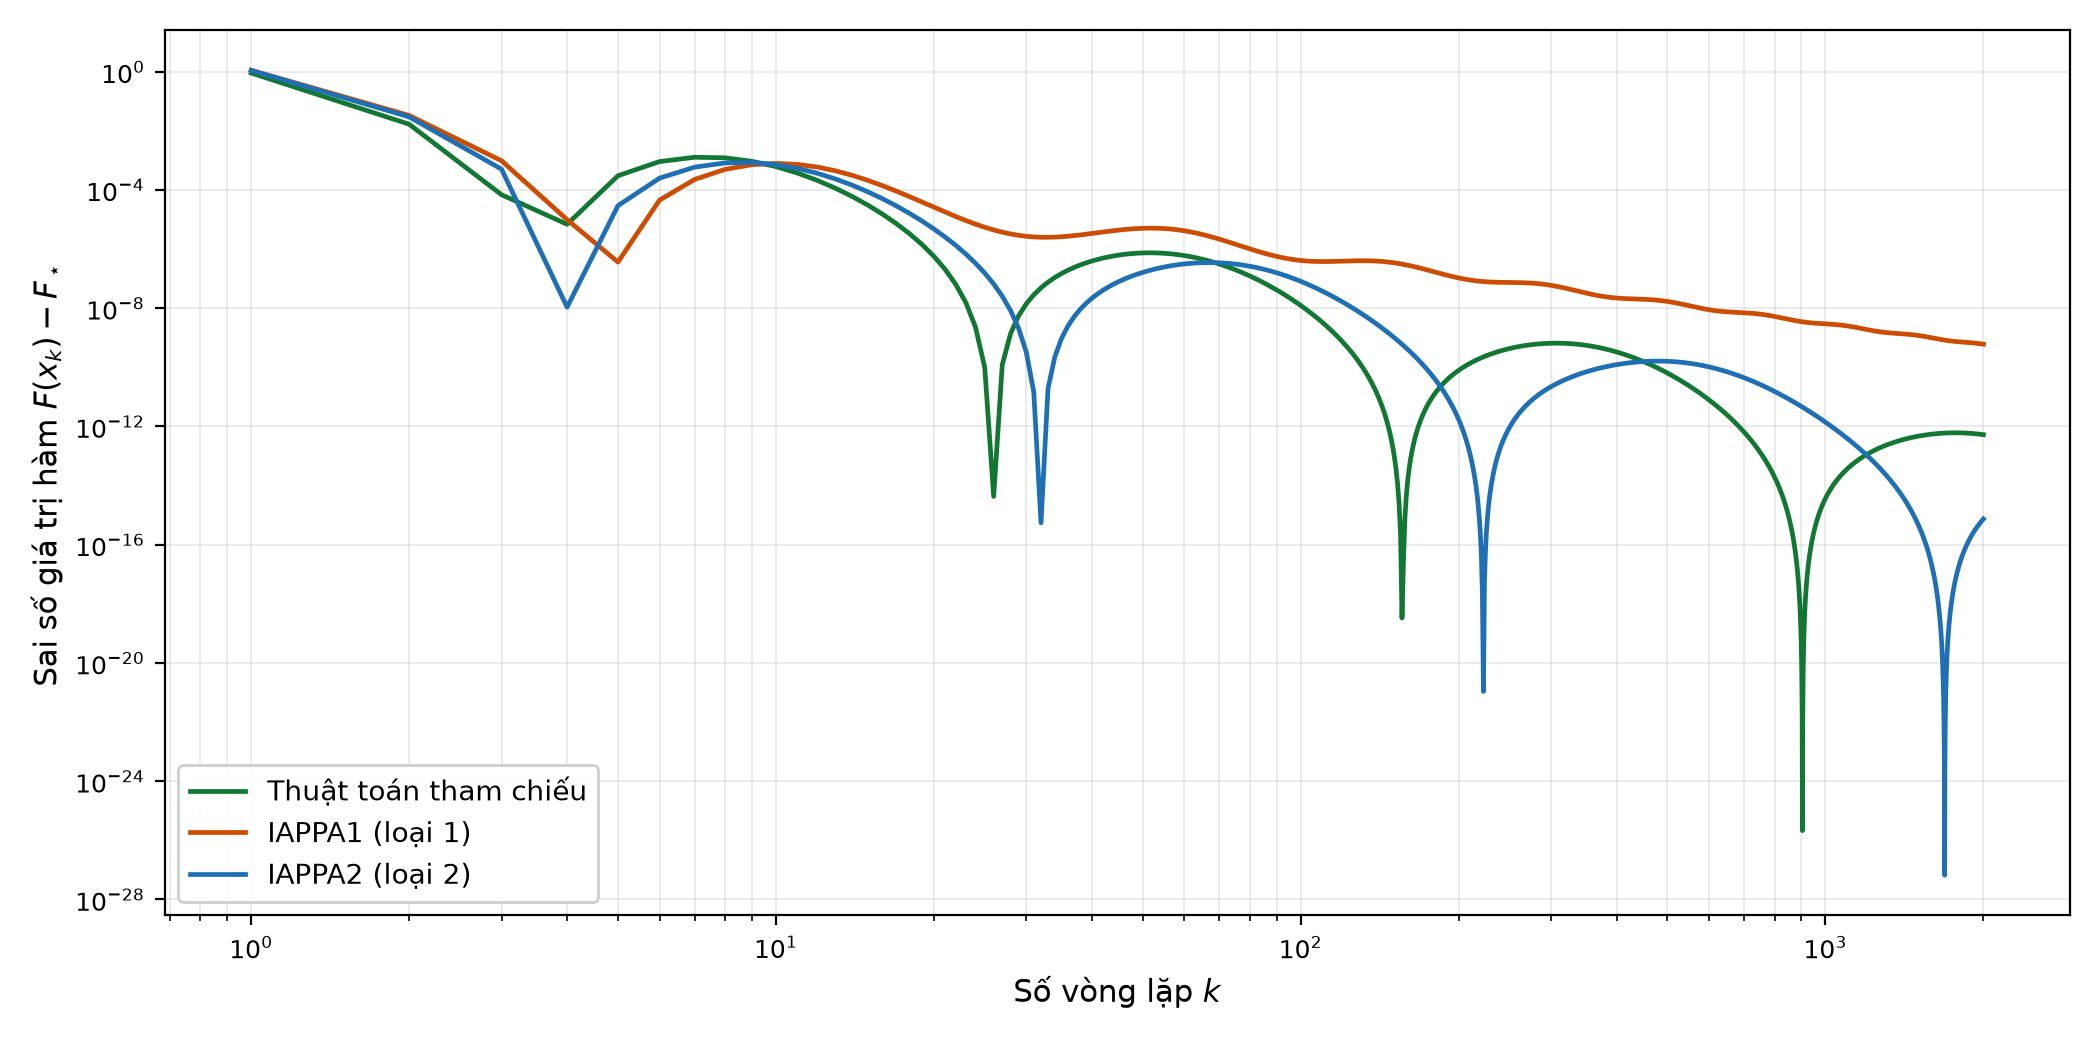
\includegraphics[width=0.90\textwidth]{figures/quartic-objective-convergence.png}
\caption{Sai số giá trị hàm trên hệ trục log--log.}
\label{fig:objective}
\end{figure}
\FloatBarrier

Hình \ref{fig:objective} cho thấy cả ba dãy giá trị hàm đều tiến về $F_{\star}$. IAPPA1 giảm chậm hơn ở giai đoạn cuối. Quỹ đạo IAPPA2 có thể nằm dưới quỹ đạo tham chiếu vì phép tính gần đúng làm thay đổi cả điểm hiện tại và điểm ngoại suy; hiện tượng này không tạo ra một chặn lý thuyết mạnh hơn phương pháp tham chiếu.

\begin{figure}[H]
\centering
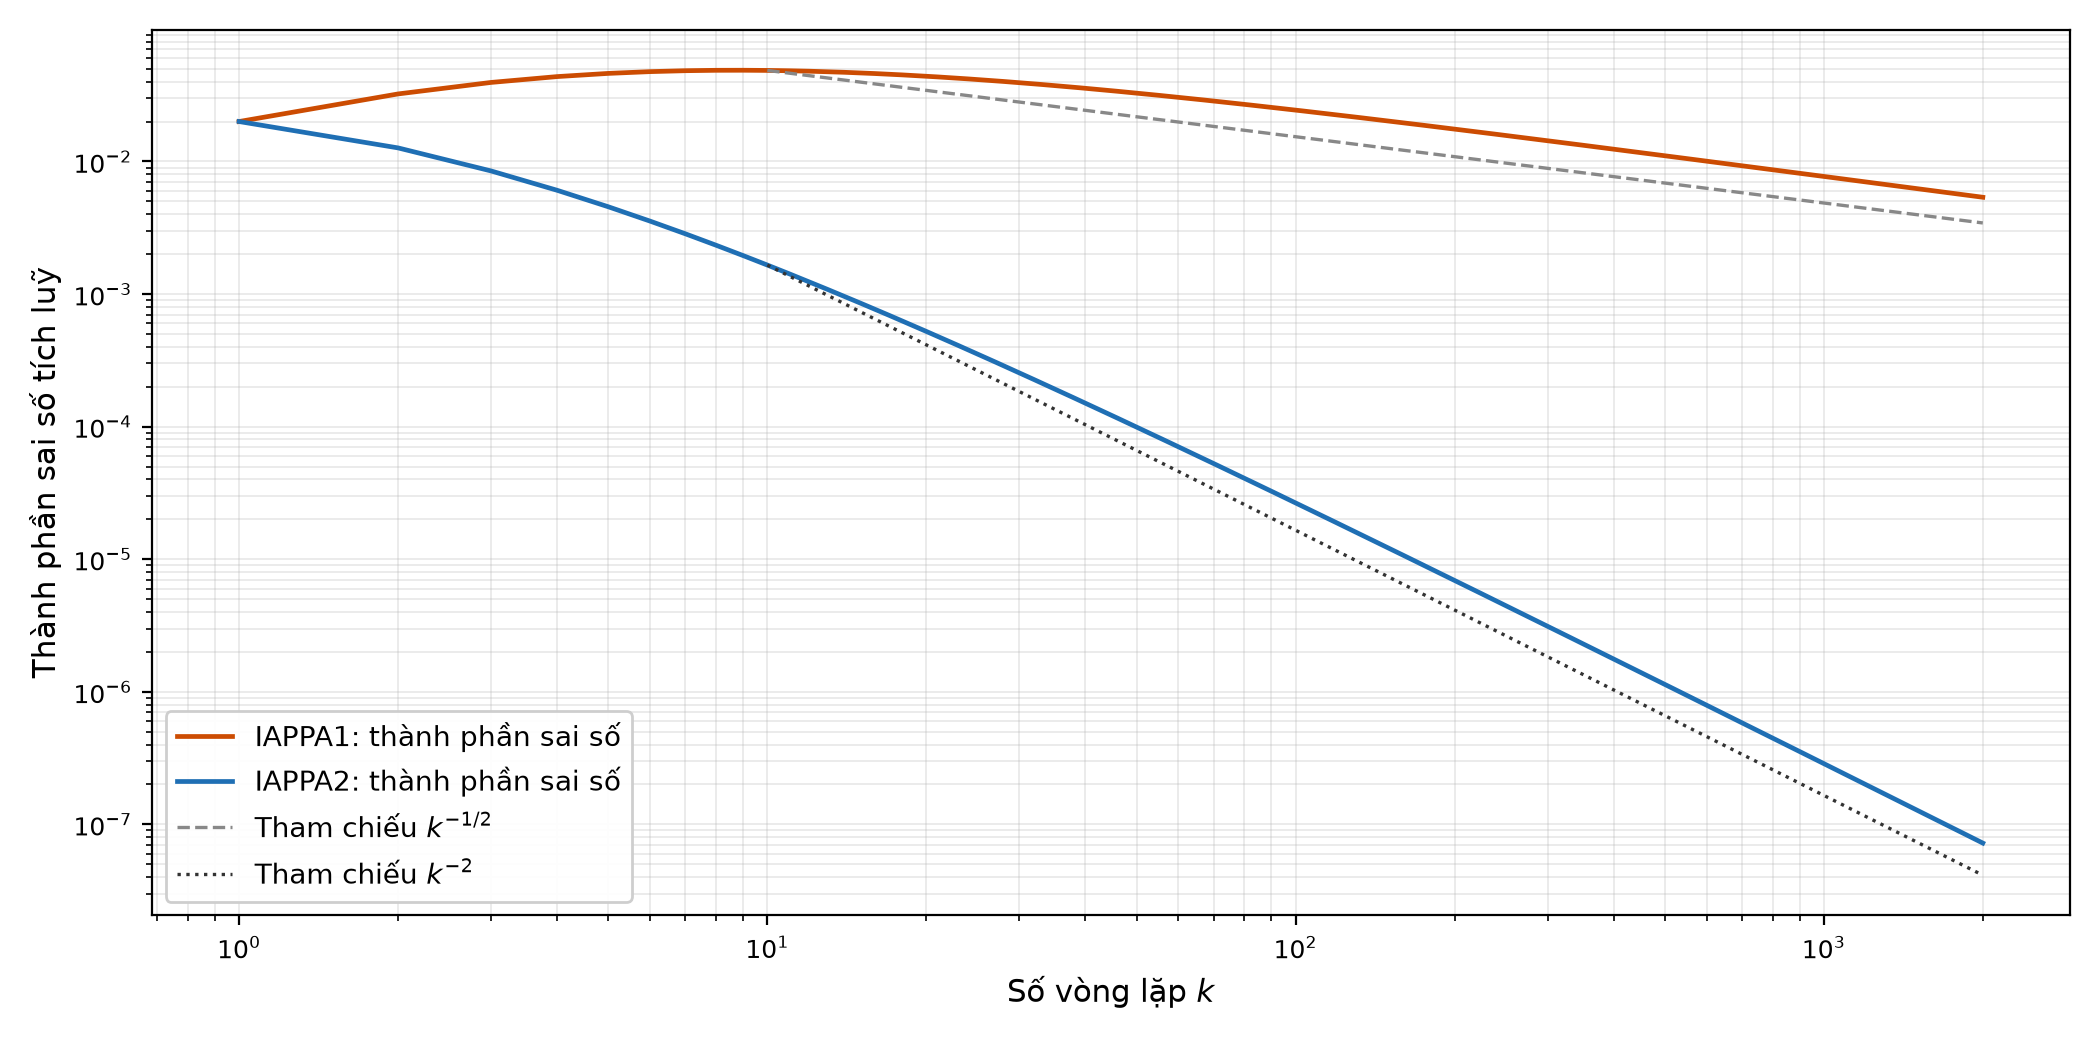
\includegraphics[width=0.90\textwidth]{figures/quartic-error-accumulation.png}
\caption{Hai thành phần sai số tích lũy $\delta_k$ trên hệ trục log--log.}
\label{fig:error}
\end{figure}
\FloatBarrier

Với $q=7/4$, Định lý 5.1 cho bậc $k^{-1/2}$ đối với chặn của IAPPA1, trong khi Định lý 5.2 cho bậc $k^{-2}$ đối với IAPPA2. Hồi quy tuyến tính của $\log\delta_k$ theo $\log k$ trên đoạn $500\leq k\leq2000$ cho hai hệ số góc lần lượt là $-0.521$ và $-1.989$. Hai giá trị này gần với các số mũ dự đoán $-1/2$ và $-2$.

\begin{table}[H]
\centering
\caption{Kết quả sau $2000$ vòng lặp.}
\label{tab:results}
\renewcommand{\arraystretch}{1.25}
\setlength{\tabcolsep}{4pt}
\small
\begin{tabular}{|>{\raggedright\arraybackslash}m{3.8cm}|>{\centering\arraybackslash}m{3.3cm}|>{\centering\arraybackslash}m{3.6cm}|>{\centering\arraybackslash}m{3.0cm}|}
\hline
\textbf{Phương pháp} & \textbf{$F(x_N)-F_{\star}$} & \textbf{Hệ số góc của $\delta_k$} & \textbf{Sai lệch cực đại $|\rho_k-1|$} \\
\hline
Thuật toán tham chiếu & $5.266\times10^{-13}$ & -- & -- \\
\hline
IAPPA1, $q=7/4$ & $6.067\times10^{-10}$ & $-0.521$ & $8.0\times10^{-12}$ \\
\hline
IAPPA2, $q=7/4$ & $7.440\times10^{-16}$ & $-1.989$ & $7.8\times10^{-10}$ \\
\hline
\end{tabular}
\end{table}

Trong Bảng \ref{tab:results}, $\rho_k$ là tỉ số giữa vế trái và ngưỡng sai số của phương trình biên tương ứng. Sai lệch nhỏ của $\rho_k$ so với $1$ phản ánh độ chính xác hữu hạn của phép giải số, đặc biệt khi ngưỡng sai số ở các vòng lặp cuối tiến gần độ chính xác máy. Thực nghiệm xác nhận tính hợp lệ của cách dựng điểm và minh họa cơ chế tích lũy sai số; nó không thay thế các chặn hội tụ tổng quát.

